%% bare_jrnl.tex
%% V1.4b
%% 2015/08/26
%% by Michael Shell
%% see http://www.michaelshell.org/
%% for current contact information.
%% Modified by Dheepak Krishnamurthy for use with Pandoc
%%
%% This is a skeleton file demonstrating the use of IEEEtran.cls
%% (requires IEEEtran.cls version 1.8b or later) with an IEEE
%% journal paper.
%%
%% Support sites:
%% http://www.michaelshell.org/tex/ieeetran/
%% http://www.ctan.org/pkg/ieeetran
%% and
%% http://www.ieee.org/

%%*************************************************************************
%% Legal Notice:
%% This code is offered as-is without any warranty either expressed or
%% implied; without even the implied warranty of MERCHANTABILITY or
%% FITNESS FOR A PARTICULAR PURPOSE!
%% User assumes all risk.
%% In no event shall the IEEE or any contributor to this code be liable for
%% any damages or losses, including, but not limited to, incidental,
%% consequential, or any other damages, resulting from the use or misuse
%% of any information contained here.
%%
%% All comments are the opinions of their respective authors and are not
%% necessarily endorsed by the IEEE.
%%
%% This work is distributed under the LaTeX Project Public License (LPPL)
%% ( http://www.latex-project.org/ ) version 1.3, and may be freely used,
%% distributed and modified. A copy of the LPPL, version 1.3, is included
%% in the base LaTeX documentation of all distributions of LaTeX released
%% 2003/12/01 or later.
%% Retain all contribution notices and credits.
%% ** Modified files should be clearly indicated as such, including  **
%% ** renaming them and changing author support contact information. **
%%*************************************************************************


% *** Authors should verify (and, if needed, correct) their LaTeX system  ***
% *** with the testflow diagnostic prior to trusting their LaTeX platform ***
% *** with production work. The IEEE's font choices and paper sizes can   ***
% *** trigger bugs that do not appear when using other class files.       ***                          ***
% The testflow support page is at:
% http://www.michaelshell.org/tex/testflow/



\documentclass[journal,]{IEEEtran}
%
% If IEEEtran.cls has not been installed into the LaTeX system files,
% manually specify the path to it like:
% \documentclass[journal]{../sty/IEEEtran}

% Some very useful LaTeX packages include:
% (uncomment the ones you want to load)


% *** MISC UTILITY PACKAGES ***
%
%\usepackage{ifpdf}
% Heiko Oberdiek's ifpdf.sty is very useful if you need conditional
% compilation based on whether the output is pdf or dvi.
% usage:
% \ifpdf
%   % pdf code
% \else
%   % dvi code
% \fi
% The latest version of ifpdf.sty can be obtained from:
% http://www.ctan.org/pkg/ifpdf
% Also, note that IEEEtran.cls V1.7 and later provides a builtin
% \ifCLASSINFOpdf conditional that works the same way.
% When switching from latex to pdflatex and vice-versa, the compiler may
% have to be run twice to clear warning/error messages.






% *** CITATION PACKAGES ***
%
%\usepackage{cite}
% cite.sty was written by Donald Arseneau
% V1.6 and later of IEEEtran pre-defines the format of the cite.sty package
% \cite{} output to follow that of the IEEE. Loading the cite package will
% result in citation numbers being automatically sorted and properly
% "compressed/ranged". e.g., [1], [9], [2], [7], [5], [6] without using
% cite.sty will become [1], [2], [5]--[7], [9] using cite.sty. cite.sty's
% \cite will automatically add leading space, if needed. Use cite.sty's
% noadjust option (cite.sty V3.8 and later) if you want to turn this off
% such as if a citation ever needs to be enclosed in parenthesis.
% cite.sty is already installed on most LaTeX systems. Be sure and use
% version 5.0 (2009-03-20) and later if using hyperref.sty.
% The latest version can be obtained at:
% http://www.ctan.org/pkg/cite
% The documentation is contained in the cite.sty file itself.






% *** GRAPHICS RELATED PACKAGES ***
%
\ifCLASSINFOpdf
  % \usepackage[pdftex]{graphicx}
  % declare the path(s) where your graphic files are
  % \graphicspath{{../pdf/}{../jpeg/}}
  % and their extensions so you won't have to specify these with
  % every instance of \includegraphics
  % \DeclareGraphicsExtensions{.pdf,.jpeg,.png}
\else
  % or other class option (dvipsone, dvipdf, if not using dvips). graphicx
  % will default to the driver specified in the system graphics.cfg if no
  % driver is specified.
  % \usepackage[dvips]{graphicx}
  % declare the path(s) where your graphic files are
  % \graphicspath{{../eps/}}
  % and their extensions so you won't have to specify these with
  % every instance of \includegraphics
  % \DeclareGraphicsExtensions{.eps}
\fi
% graphicx was written by David Carlisle and Sebastian Rahtz. It is
% required if you want graphics, photos, etc. graphicx.sty is already
% installed on most LaTeX systems. The latest version and documentation
% can be obtained at:
% http://www.ctan.org/pkg/graphicx
% Another good source of documentation is "Using Imported Graphics in
% LaTeX2e" by Keith Reckdahl which can be found at:
% http://www.ctan.org/pkg/epslatex
%
% latex, and pdflatex in dvi mode, support graphics in encapsulated
% postscript (.eps) format. pdflatex in pdf mode supports graphics
% in .pdf, .jpeg, .png and .mps (metapost) formats. Users should ensure
% that all non-photo figures use a vector format (.eps, .pdf, .mps) and
% not a bitmapped formats (.jpeg, .png). The IEEE frowns on bitmapped formats
% which can result in "jaggedy"/blurry rendering of lines and letters as
% well as large increases in file sizes.
%
% You can find documentation about the pdfTeX application at:
% http://www.tug.org/applications/pdftex





% *** MATH PACKAGES ***
%
%\usepackage{amsmath}
% A popular package from the American Mathematical Society that provides
% many useful and powerful commands for dealing with mathematics.
%
% Note that the amsmath package sets \interdisplaylinepenalty to 10000
% thus preventing page breaks from occurring within multiline equations. Use:
%\interdisplaylinepenalty=2500
% after loading amsmath to restore such page breaks as IEEEtran.cls normally
% does. amsmath.sty is already installed on most LaTeX systems. The latest
% version and documentation can be obtained at:
% http://www.ctan.org/pkg/amsmath





% *** SPECIALIZED LIST PACKAGES ***
%
%\usepackage{algorithmic}
% algorithmic.sty was written by Peter Williams and Rogerio Brito.
% This package provides an algorithmic environment fo describing algorithms.
% You can use the algorithmic environment in-text or within a figure
% environment to provide for a floating algorithm. Do NOT use the algorithm
% floating environment provided by algorithm.sty (by the same authors) or
% algorithm2e.sty (by Christophe Fiorio) as the IEEE does not use dedicated
% algorithm float types and packages that provide these will not provide
% correct IEEE style captions. The latest version and documentation of
% algorithmic.sty can be obtained at:
% http://www.ctan.org/pkg/algorithms
% Also of interest may be the (relatively newer and more customizable)
% algorithmicx.sty package by Szasz Janos:
% http://www.ctan.org/pkg/algorithmicx




% *** ALIGNMENT PACKAGES ***
%
%\usepackage{array}
% Frank Mittelbach's and David Carlisle's array.sty patches and improves
% the standard LaTeX2e array and tabular environments to provide better
% appearance and additional user controls. As the default LaTeX2e table
% generation code is lacking to the point of almost being broken with
% respect to the quality of the end results, all users are strongly
% advised to use an enhanced (at the very least that provided by array.sty)
% set of table tools. array.sty is already installed on most systems. The
% latest version and documentation can be obtained at:
% http://www.ctan.org/pkg/array


% IEEEtran contains the IEEEeqnarray family of commands that can be used to
% generate multiline equations as well as matrices, tables, etc., of high
% quality.




% *** SUBFIGURE PACKAGES ***
%\ifCLASSOPTIONcompsoc
%  \usepackage[caption=false,font=normalsize,labelfont=sf,textfont=sf]{subfig}
%\else
%  \usepackage[caption=false,font=footnotesize]{subfig}
%\fi
% subfig.sty, written by Steven Douglas Cochran, is the modern replacement
% for subfigure.sty, the latter of which is no longer maintained and is
% incompatible with some LaTeX packages including fixltx2e. However,
% subfig.sty requires and automatically loads Axel Sommerfeldt's caption.sty
% which will override IEEEtran.cls' handling of captions and this will result
% in non-IEEE style figure/table captions. To prevent this problem, be sure
% and invoke subfig.sty's "caption=false" package option (available since
% subfig.sty version 1.3, 2005/06/28) as this is will preserve IEEEtran.cls
% handling of captions.
% Note that the Computer Society format requires a larger sans serif font
% than the serif footnote size font used in traditional IEEE formatting
% and thus the need to invoke different subfig.sty package options depending
% on whether compsoc mode has been enabled.
%
% The latest version and documentation of subfig.sty can be obtained at:
% http://www.ctan.org/pkg/subfig




% *** FLOAT PACKAGES ***
%
%\usepackage{fixltx2e}
% fixltx2e, the successor to the earlier fix2col.sty, was written by
% Frank Mittelbach and David Carlisle. This package corrects a few problems
% in the LaTeX2e kernel, the most notable of which is that in current
% LaTeX2e releases, the ordering of single and double column floats is not
% guaranteed to be preserved. Thus, an unpatched LaTeX2e can allow a
% single column figure to be placed prior to an earlier double column
% figure.
% Be aware that LaTeX2e kernels dated 2015 and later have fixltx2e.sty's
% corrections already built into the system in which case a warning will
% be issued if an attempt is made to load fixltx2e.sty as it is no longer
% needed.
% The latest version and documentation can be found at:
% http://www.ctan.org/pkg/fixltx2e


%\usepackage{stfloats}
% stfloats.sty was written by Sigitas Tolusis. This package gives LaTeX2e
% the ability to do double column floats at the bottom of the page as well
% as the top. (e.g., "\begin{figure*}[!b]" is not normally possible in
% LaTeX2e). It also provides a command:
%\fnbelowfloat
% to enable the placement of footnotes below bottom floats (the standard
% LaTeX2e kernel puts them above bottom floats). This is an invasive package
% which rewrites many portions of the LaTeX2e float routines. It may not work
% with other packages that modify the LaTeX2e float routines. The latest
% version and documentation can be obtained at:
% http://www.ctan.org/pkg/stfloats
% Do not use the stfloats baselinefloat ability as the IEEE does not allow
% \baselineskip to stretch. Authors submitting work to the IEEE should note
% that the IEEE rarely uses double column equations and that authors should try
% to avoid such use. Do not be tempted to use the cuted.sty or midfloat.sty
% packages (also by Sigitas Tolusis) as the IEEE does not format its papers in
% such ways.
% Do not attempt to use stfloats with fixltx2e as they are incompatible.
% Instead, use Morten Hogholm'a dblfloatfix which combines the features
% of both fixltx2e and stfloats:
%
% \usepackage{dblfloatfix}
% The latest version can be found at:
% http://www.ctan.org/pkg/dblfloatfix




%\ifCLASSOPTIONcaptionsoff
%  \usepackage[nomarkers]{endfloat}
% \let\MYoriglatexcaption\caption
% \renewcommand{\caption}[2][\relax]{\MYoriglatexcaption[#2]{#2}}
%\fi
% endfloat.sty was written by James Darrell McCauley, Jeff Goldberg and
% Axel Sommerfeldt. This package may be useful when used in conjunction with
% IEEEtran.cls'  captionsoff option. Some IEEE journals/societies require that
% submissions have lists of figures/tables at the end of the paper and that
% figures/tables without any captions are placed on a page by themselves at
% the end of the document. If needed, the draftcls IEEEtran class option or
% \CLASSINPUTbaselinestretch interface can be used to increase the line
% spacing as well. Be sure and use the nomarkers option of endfloat to
% prevent endfloat from "marking" where the figures would have been placed
% in the text. The two hack lines of code above are a slight modification of
% that suggested by in the endfloat docs (section 8.4.1) to ensure that
% the full captions always appear in the list of figures/tables - even if
% the user used the short optional argument of \caption[]{}.
% IEEE papers do not typically make use of \caption[]'s optional argument,
% so this should not be an issue. A similar trick can be used to disable
% captions of packages such as subfig.sty that lack options to turn off
% the subcaptions:
% For subfig.sty:
% \let\MYorigsubfloat\subfloat
% \renewcommand{\subfloat}[2][\relax]{\MYorigsubfloat[]{#2}}
% However, the above trick will not work if both optional arguments of
% the \subfloat command are used. Furthermore, there needs to be a
% description of each subfigure *somewhere* and endfloat does not add
% subfigure captions to its list of figures. Thus, the best approach is to
% avoid the use of subfigure captions (many IEEE journals avoid them anyway)
% and instead reference/explain all the subfigures within the main caption.
% The latest version of endfloat.sty and its documentation can obtained at:
% http://www.ctan.org/pkg/endfloat
%
% The IEEEtran \ifCLASSOPTIONcaptionsoff conditional can also be used
% later in the document, say, to conditionally put the References on a
% page by themselves.




% *** PDF, URL AND HYPERLINK PACKAGES ***
%
%\usepackage{url}
% url.sty was written by Donald Arseneau. It provides better support for
% handling and breaking URLs. url.sty is already installed on most LaTeX
% systems. The latest version and documentation can be obtained at:
% http://www.ctan.org/pkg/url
% Basically, \url{my_url_here}.


% *** Do not adjust lengths that control margins, column widths, etc. ***
% *** Do not use packages that alter fonts (such as pslatex).         ***
% There should be no need to do such things with IEEEtran.cls V1.6 and later.
% (Unless specifically asked to do so by the journal or conference you plan
% to submit to, of course. )

% correct bad hyphenation here

% Pandoc template fixes

\usepackage{lmodern}
\usepackage{amssymb,amsmath}
\usepackage{ifxetex,ifluatex}
\usepackage{fixltx2e} % provides \textsubscript
\ifnum 0\ifxetex 1\fi\ifluatex 1\fi=0 % if pdftex
  \usepackage[T1]{fontenc}
  \usepackage[utf8]{inputenc}
\else % if luatex or xelatex
  \ifxetex
    \usepackage{mathspec}
  \else
    \usepackage{fontspec}
  \fi
  \defaultfontfeatures{Ligatures=TeX,Scale=MatchLowercase}
\fi
% use upquote if available, for straight quotes in verbatim environments
\IfFileExists{upquote.sty}{\usepackage{upquote}}{}
% use microtype if available
\IfFileExists{microtype.sty}{%
\usepackage{microtype}
\UseMicrotypeSet[protrusion]{basicmath} % disable protrusion for tt fonts
}{}
\usepackage{hyperref}
\hypersetup{unicode=true,
            pdftitle={Writing Technical Papers with Markdown and Pandoc},
            pdfkeywords={markdown, pandoc, papers, writing, academic,
scholarly, technical, scientific},
            pdfborder={0 0 0},
            breaklinks=true}
\urlstyle{same}  % don't use monospace font for urls
\usepackage{longtable,booktabs}
\makeatletter
\let\oldlt\longtable
\let\endoldlt\endlongtable
\def\longtable{\@ifnextchar[\longtable@i \longtable@ii}
\def\longtable@i[#1]{\begin{figure}[t]
\onecolumn
\begin{minipage}{0.5\textwidth}
\oldlt[#1]
}
\def\longtable@ii{\begin{figure}[t]
\onecolumn
\begin{minipage}{0.5\textwidth}
\oldlt
}
\def\endlongtable{\endoldlt
\end{minipage}
\twocolumn
\end{figure}}
\makeatother
\usepackage{graphicx,grffile}
\makeatletter
\def\maxwidth{\ifdim\Gin@nat@width>\linewidth\linewidth\else\Gin@nat@width\fi}
\def\maxheight{\ifdim\Gin@nat@height>\textheight\textheight\else\Gin@nat@height\fi}
\makeatother
% Scale images if necessary, so that they will not overflow the page
% margins by default, and it is still possible to overwrite the defaults
% using explicit options in \includegraphics[width, height, ...]{}
\setkeys{Gin}{width=\maxwidth,height=\maxheight,keepaspectratio}
\usepackage[normalem]{ulem}
% avoid problems with \sout in headers with hyperref:
\pdfstringdefDisableCommands{\renewcommand{\sout}{}}
\IfFileExists{parskip.sty}{%
\usepackage{parskip}
}{% else
\setlength{\parindent}{0pt}
\setlength{\parskip}{6pt plus 2pt minus 1pt}
}
\setlength{\emergencystretch}{3em}  % prevent overfull lines
\providecommand{\tightlist}{%
  \setlength{\itemsep}{0pt}\setlength{\parskip}{0pt}}
\setcounter{secnumdepth}{0}
% Redefines (sub)paragraphs to behave more like sections
\ifx\paragraph\undefined\else
\let\oldparagraph\paragraph
\renewcommand{\paragraph}[1]{\oldparagraph{#1}\mbox{}}
\fi
\ifx\subparagraph\undefined\else
\let\oldsubparagraph\subparagraph
\renewcommand{\subparagraph}[1]{\oldsubparagraph{#1}\mbox{}}
\fi

%%%% pandoc-fignos: required package
\usepackage{caption}

%% pandoc-fignos: environment to disable figure caption prefixes
\makeatletter
\newcounter{figno}
\newenvironment{fignos:no-prefix-figure-caption}{
  \caption@ifcompatibility{}{
    \let\oldthefigure\thefigure
    \let\oldtheHfigure\theHfigure
    \renewcommand{\thefigure}{figno:\thefigno}
    \renewcommand{\theHfigure}{figno:\thefigno}
    \stepcounter{figno}
    \captionsetup{labelformat=empty}
  }
}{
  \caption@ifcompatibility{}{
    \captionsetup{labelformat=default}
    \let\thefigure\oldthefigure
    \let\theHfigure\oldtheHfigure
    \addtocounter{figure}{-1}
  }
}
\makeatother

%% pandoc-tablenos: environment to disable table caption prefixes
\makeatletter
\newcounter{tableno}
\newenvironment{tablenos:no-prefix-table-caption}{
  \caption@ifcompatibility{}{
    \let\oldthetable\thetable
    \let\oldtheHtable\theHtable
    \renewcommand{\thetable}{tableno:\thetableno}
    \renewcommand{\theHtable}{tableno:\thetableno}
    \stepcounter{tableno}
    \captionsetup{labelformat=empty}
  }
}{
  \caption@ifcompatibility{}{
    \captionsetup{labelformat=default}
    \let\thetable\oldthetable
    \let\theHtable\oldtheHtable
    \addtocounter{table}{-1}
  }
}
\makeatother


\begin{document}

\title{\bigskip \bigskip Writing Technical Papers with Markdown and
Pandoc}


% The paper headers
% The only time the second header will appear is for the odd numbered pages
% after the title page when using the twoside option.
%
% *** Note that you probably will NOT want to include the author's ***
% *** name in the headers of peer review papers.                   ***
% You can use \ifCLASSOPTIONpeerreview for conditional compilation here if
% you desire.




% If you want to put a publisher's ID mark on the page you can do it like
% this:
%
% Remember, if you use this you must call \IEEEpubidadjcol in the second
% column for its text to clear the IEEEpubid mark.

% use for special paper notices
%\IEEEspecialpapernotice{(Invited Paper)}




% make the title area
\maketitle

% As a general rule, do not put math, special symbols or citations
% in the abstract or keywords.

\begin{abstract}

\noindent Recently, I've had several people ask me about the Markdown
workflow I use to write papers. I figured I'd use this post to write
about my workflow and my resources on this topic.

\end{abstract}


% Note that keywords are not normally used for peerreview papers.

% page as needed:
% \ifCLASSOPTIONpeerreview
% \begin{center} \bfseries EDICS Category: 3-BBND \end{center}
% \fi
%
% For peerreview papers, this IEEEtran command inserts a page break and
% creates the second title. It will be ignored for other modes.
\IEEEpeerreviewmaketitle

You can view this post in the following formats, thanks to Pandoc!

\begin{tablenos:no-prefix-table-caption}

\begin{longtable}[]{@{}ll@{}}
\toprule
Format & Link\tabularnewline
\midrule
\endhead
IEEE-PDF &
\href{https://blog.kdheepak.com/downloads/writing-papers-with-markdown.ieee.pdf}{LINK}\tabularnewline
IEEE-DOCX &
\href{https://blog.kdheepak.com/downloads/writing-papers-with-markdown.ieee.docx}{LINK}\tabularnewline
IEEE-HTML &
\href{https://blog.kdheepak.com/downloads/writing-papers-with-markdown.ieee.html}{LINK}\tabularnewline
PDF &
\href{https://blog.kdheepak.com/downloads/writing-papers-with-markdown.pdf}{LINK}\tabularnewline
DOCX &
\href{https://blog.kdheepak.com/downloads/writing-papers-with-markdown.docx}{LINK}\tabularnewline
HTML &
\href{https://blog.kdheepak.com/downloads/writing-papers-with-markdown.html}{LINK}\tabularnewline
SLIDES-PDF &
\href{https://blog.kdheepak.com/downloads/writing-papers-with-markdown.slides.pdf}{LINK}\tabularnewline
\bottomrule
\end{longtable}

\end{tablenos:no-prefix-table-caption}

\begin{IEEEkeywords}
Pandoc, LaTeX, Markdown
\end{IEEEkeywords}

I've had several people ask me about Markdown for academic writing
recently. I figured I'd use this post to write about my workflow and my
resources on this topic.

\hypertarget{why-markdown}{%
\section{Why Markdown}\label{why-markdown}}

Academic writing involves:

\begin{itemize}
\tightlist
\item
  writing down ideas as they come along and documenting results
  (notetaking),
\item
  experimenting with these ideas (simulations and data analysis),
\item
  and finally presenting them effectively (scientific paper).
\end{itemize}

There's a lot to manage over the length of time this entire process
spans. Academics require a set of tools that aid in making this process,
i.e.~the effective communication of ideas, as seamless as possible.
There are currently two popular options for academics seeking to write
technical papers - Microsoft Word or \(\LaTeX\).

\hypertarget{a-word-about-word}{%
\subsection{A word about Word}\label{a-word-about-word}}

Microsoft Word is ubiquitous when it comes to writing reports. The great
thing about Word is that there is almost no barrier to \emph{begin}
writing. You can incrementally build your skill in using this tool as
and when you are using it. This is useful since it makes it immediately
accessible, thereby decreasing the time and effort spent on learning how
to use a software for writing and allowing you to concentrate on the
writing itself.

However, I've found a few fundamental problems with Microsoft Word.
Having a WYSIWYG (What You See Is What You Get) editor is great (even
Richard Stallman seems to think so
{[}\protect\hyperlink{ref-stallman_emacs_nodate}{1}{]}). However,
products like Word fail miserably at separating content from formatting.
These products impose on the writer their own concept of how a document
should be formatted, which I've found greatly hinders the writing
process. Have you ever experienced a sudden jump in spacing? Or
mismatched formatting after a copy and paste from one part of the
document to another? Or have indents and bullet points misbehave
haphazardly? Word applies these formatting changes seemingly at random!
These are all typesetting and formatting processes and these should be
applied \textbf{\emph{after}} the text is completed. These processes
should not distract from the task at hand\footnote{I understand that
  there may be more \emph{correct} ways to go about it, I just don't
  want to be thinking about all that while I'm writing.} - writing!

There are other issues as well. Microsoft's ecosystem comes at a price,
literally. Word is proprietary, and Word's format is a proprietary data
format. When you use Word, by storing your work in this proprietary
software's proprietary data format, you tie yourself down to this
particular licensed software for the forseeable future. You also make
the implicit assumption that everyone you work with has the same
software on their computer. Word also does not play well with its
counterparts on OSX. With the same content, the document is presented
differently depending on which machine you open it on. As far as I know
there isn't even a version for Linux machines. Heck, Microsoft Word does
not even play well with previous versions of Microsoft Word. I
understand why this issue occurs, considering the complexity in
operating systems and software. Backward incompatible software or cross
incompatibility are probably inevitable, but as an user, I shouldn't
have to be concerned about this. I shouldn't have to think about what
software or what version of a software my reviewers are using when I'm
sending them a document. And speaking of sharing documents, did you know
you can end up transferring malware through a Word document? Just think
about that for a second. Opening what should be essentially a text file
is a security risk for your machine. And some of these viruses (as of
the time of this writing) do not even have patches yet
{[}\protect\hyperlink{ref-beaumont_bypass_2015}{2}{]}. Loads of people
have already talked about this and similar issues at some length
{[}\protect\hyperlink{ref-steingold_proprietary_nodate}{3}{]},
{[}\protect\hyperlink{ref-cottrell_word_nodate}{4}{]}, and have probably
done more justice to this topic that I possibly could. With all these
issues, it is hard to believe Word is so widely accepted as a standard.

I think there is a strong case to be made about why you should consider
dropping Word for your next paper. In addition to what has been
discussed above:

\begin{itemize}
\tightlist
\item
  Word is slow, and consumes sometimes up to a gig of virtual memory.
  For what is basically a word processor, that is unnecessary.
\item
  there is no clean way to permanently save comments or notes, that
  persist in the final version without affecting how final document
  looks.
\item
  collaborating with other people requires foresight and planning.
\item
  the equation editor is painful to use.
\item
  Word does not work in the workflow for \textbf{scientific research
  papers or reports}.
\end{itemize}

Let us assume that scientific research papers consists of only 3 steps
(if only!) - notetaking, analysis and presentation. Word fails at
delivering at all these tasks. Word doesn't quite work for notetaking.
Org mode, Evernote or Onenote are most people's preferred solution. Word
doesn't fit data analysis requirements as well, with Python, R or Excel
being the go-to tools. I personally use Emacs / Vim for notetaking and
store them in a git repository and all of my data analysis is done in
Jupyter Notebooks. After collecting the required data from an experiment
and post-processing it, I can save plots into an image or the data into
a table in a particular format programmatically using scripts. Word
however, does not allow me to import these images or tables
programmatically. If I did somehow manage to contort my workflow and
store my data and information in this software, I have absolutely no way
of retrieving it. The final presentation/report/paper, information and
data will exist confined in this closed source proprietary software.
Word just does not fit into an analysis or research workflow. To quote
Raymond Hettinger:

\begin{fignos:no-prefix-figure-caption}

\begin{figure}
\centering
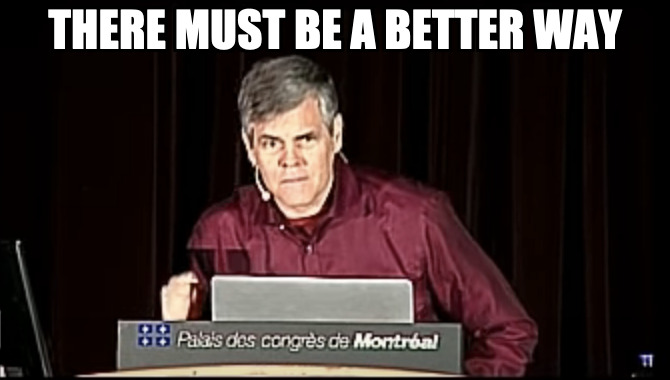
\includegraphics{images/raymondhettinger.jpg}
\caption{Raymond Hettinger}
\end{figure}

\end{fignos:no-prefix-figure-caption}

\hypertarget{latex---lah-tekh-lah-tek-or-lay-tek}{%
\subsection{\texorpdfstring{\(\LaTeX\) - lah-tekh, lah-tek or
lay-tek}{\textbackslash LaTeX - lah-tekh, lah-tek or lay-tek}}\label{latex---lah-tekh-lah-tek-or-lay-tek}}

Enter \(\LaTeX\).

\begin{quote}
\(\LaTeX\) is to a book what a set of blueprints is to a building.
{[}\protect\hyperlink{ref-noauthor_stackoverflow_nodate}{5}{]}
\end{quote}

\(\LaTeX\) is a typesetting system and is frequently used in scientific,
technical and mathematical papers. It is infamous for displaying
equations in a manner that looks great. Math is beautiful, and it
deserves to be presented beautifully.

\begin{align}
  \hskip6em \nabla \times \vec{\mathbf{B}} -\, \frac1c\, \frac{\partial\vec{\mathbf{E}}}{\partial t} & = \frac{4\pi}{c}\vec{\mathbf{j}} \hskip6em \\
  \nabla \cdot \vec{\mathbf{E}} & = 4 \pi \rho \\
  \nabla \times \vec{\mathbf{E}}\, +\, \frac1c\, \frac{\partial\vec{\mathbf{B}}}{\partial t} & = \vec{\mathbf{0}} \\
  \nabla \cdot \vec{\mathbf{B}} & = 0
\end{align}

Essentially, \(\LaTeX\) is a markup language. Content is written in
plain text and can be annotated with commands that describe how certain
elements should be displayed.

For example, take a look at the following commands.

\begin{verbatim}
\textbf{bold}
\textit{italic}
\end{verbatim}

This markup will format the words passed into these ``functions'' as
\textbf{bold} and \emph{italic} respectively.

There are numerous similar functions for different aspects of
formatting. This allows you to concentrate on writing, without worrying
about the typesetting until later.

The source document that contains the content is a plain text file. This
means you can use \texttt{git} to version control the paper. This allows
you to track changes and collaborate with others without any additional
effort. This also lets you work with your favourite text editor - Vim,
Emacs, Atom. There are even TeX specific ones, such as TeXShop and Lyx.

\(\LaTeX\) is free. Free as in beer and free as in freedom. You can have
the confidence that your code and documents can survive possibly forever
in its current format. The \(\LaTeX\) community is great and are very
helpful towards beginners. There are hundreds of packages that improve
upon the functionality that \(\LaTeX\) provides. There are packages like
\emph{TikZ} that let you to create high resolution print quality
detailed diagrams, which I've seen used even outside a \(\LaTeX\)
environment.

However, there is a barrier to entry which one must overcome in order to
begin using \(\LaTeX\). Unlike Word, you have to know which commands are
used for what markup functionality, not only to know when to use them,
but also when not to use them. The biggest problem with \(\LaTeX\) is
probably the error messages. Most of the time they are near useless, and
sometimes they are even borderline cryptic.

Personally, I found learning how to work with \(\LaTeX\) extremely
useful. It challenged me to think about the structure of a document, and
how I could convey information effectively not just through the final
document, but also in the source material\footnote{Having the ability to
  leave comments to myself or fellow collaborators that are filtered out
  of the final presentation can be very useful.}. I also didn't think it
was difficult. Solutions to my initial problems were only a quick Google
search away. Tables were frustrating at first, but you get the hang of
them over time. Equations are a joy to type in \(\LaTeX\). And the final
product looks great!

That said, the markup language is a bit too heavy for notetaking, and
not particularly readable. For example, take a look at the syntax for a
creating a section, a subsection and list of items with some bold and
italic elements.

\begin{verbatim}
\section{Section Name}
This is text in the section
\subsection{Sub Section Name}
The following is a list in this subsection
\begin{enumerate}
  \item The first \textbf{bold} item
  \begin{enumerate}
    \item Nested item 1
    \item Nested item 2
  \end{enumerate}
  \item The second \textit{italicized} item
  \item The third etc \ldots
\end{enumerate}
\end{verbatim}

With good IDEs for \(\LaTeX\) this isn't as bad as it looks, although
they still hinder the writer's flow. Over time and with experience, one
can become proficient in \(\LaTeX\). And once you invest the time to
learn \(\LaTeX\) I can't think of any reason why you would go back to
Word. But it is likely that beginners will have a hard time getting
started. So, if you cannot afford to experiment with \(\LaTeX\), are you
resigned to Word? I don't think so. Markdown to the rescue!

\hypertarget{markdown}{%
\subsection{Markdown}\label{markdown}}

Markdown is a very lightweight easy-to-read easy-to-write plain text
markup language. The same example as before looks like this in Markdown.

\begin{verbatim}
# Section Name

This is text in the section

## Sub Section Name

The following is a list in this subsection

* The first **bold** item
    - Nested item 1
    - Nested item 2
* The second *italicized* item
* The third etc ...
\end{verbatim}

Much better! It's a lot easier to read and a lot easier to write than
\(\LaTeX\). Markdown, developed by John Gruber, was principally written
for the web, to avoid the heavy markup of HTML. Tools have been
developed to convert Markdown to HTML, PDF and even DOCX.

The main advantages of Markdown:

\begin{itemize}
\tightlist
\item
  Easy: the syntax is simple
\item
  Fast: the simple formatting saves time and speeds up workflows of
  writers
\item
  Portable: documents are cross-platform by nature
\item
  Flexible: HTML, PDF, DOCX, TEX are all supported output formats
\end{itemize}

Markdown is awesome at a set of things, and a much better alternative
than Word or \(\LaTeX\) for those specific set of things. Take for
example this table \ref{tbl:table}.

\begin{verbatim}
  Right     Left     Center     Default
-------     ------ ----------   -------
     12     12        12            12
    123     123       123          123
      1     1          1             1

Table:  Demonstration of simple table syntax.
\end{verbatim}

This is what the same table looks like in \(\LaTeX\).

\begin{verbatim}
\begin{longtable}[c]{@{}rlcl@{}}
\caption{Demonstration of simple table syntax.}
\tabularnewline
\toprule
Right & Left & Center & Default\tabularnewline
\midrule
\endfirsthead
\toprule
Right & Left & Center & Default\tabularnewline
\midrule
\endhead
12 & 12 & 12 & 12\tabularnewline
123 & 123 & 123 & 123\tabularnewline
1 & 1 & 1 & 1\tabularnewline
\bottomrule
\end{longtable}
\end{verbatim}

However, Markdown does not allow for the level of detailed customization
that you can achieve using \(\LaTeX\). Even a moderately complex table
such as the one below is not supported (currently) by any form of
Markdown.

\begin{fignos:no-prefix-figure-caption}

\begin{figure}
\centering
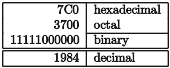
\includegraphics{images/table.png}
\caption{Tabular \(\LaTeX\) example
{[}\protect\hyperlink{ref-noauthor_wikibooks_nodate}{6}{]}}
\end{figure}

\end{fignos:no-prefix-figure-caption}

Markdown may not be as powerful as \(\LaTeX\), but its easy to write
easy to read syntax, open standard format and a strong backing from the
community make it a ideal candidate for writing. It has the advantages
of Word (ease of use) and \(\LaTeX\) (excellent typesetting) for output
formats. Also there is the added advantage of only having to write in
Markdown once, and have documents generated in a multitude of formats
later - PDF, DOCX, slides, HTML etc.

I hope that by now you are convinced that Markdown is a great tool for
writing. In the following sections we will look at how to convert a
Markdown file to other formats, and what are some potential limitations
and how you might overcome them.

\hypertarget{pandoc---a-swiss-army-knife}{%
\section{Pandoc - A ``swiss army
knife''}\label{pandoc---a-swiss-army-knife}}

Pandoc is a software tool by \href{https://johnmacfarlane.net/}{John
Macfarlane} written in Haskell that can convert a document from just
about any format to just about any other format. And works really well.

Input formats:

\begin{itemize}
\tightlist
\item
  native (native Haskell)
\item
  json (JSON version of native AST)
\item
  markdown (pandoc's extended Markdown)
\item
  markdown\_strict (original unextended Markdown)
\item
  markdown\_phpextra (PHP Markdown Extra)
\item
  markdown\_github (GitHub-Flavored Markdown)
\item
  commonmark (CommonMark Markdown)
\item
  textile (Textile)
\item
  rst (reStructuredText)
\item
  html (HTML)
\item
  docbook (DocBook)
\item
  t2t (txt2tags)
\item
  docx (docx)
\item
  odt (ODT)
\item
  epub (EPUB)
\item
  opml (OPML)
\item
  org (Emacs Org mode)
\item
  mediawiki (MediaWiki markup)
\item
  twiki (TWiki markup)
\item
  haddock (Haddock markup)
\item
  or latex (\(\LaTeX\))
\end{itemize}

Output formats:

\begin{itemize}
\tightlist
\item
  native (native Haskell)
\item
  json (JSON version of native AST)
\item
  plain (plain text)
\item
  markdown (pandoc's extended Markdown)
\item
  markdown\_strict (original unextended Markdown)
\item
  markdown\_phpextra (PHP Markdown Extra)
\item
  markdown\_github (GitHub-Flavored Markdown)
\item
  commonmark (CommonMark Markdown)
\item
  rst (reStructuredText)
\item
  html (XHTML)
\item
  html5 (HTML5)
\item
  latex (\(\LaTeX\))
\item
  beamer (\(\LaTeX\) beamer slide show)
\item
  context (ConTeXt)
\item
  man (groff man)
\item
  mediawiki (MediaWiki markup)
\item
  dokuwiki (DokuWiki markup)
\item
  textile (Textile)
\item
  org (Emacs Org mode)
\item
  texinfo (GNU Texinfo)
\item
  opml (OPML)
\item
  docbook (DocBook)
\item
  opendocument (OpenDocument)
\item
  odt (OpenOffice text document)
\item
  docx (Word docx)
\item
  haddock (Haddock markup)
\item
  rtf (rich text format)
\item
  epub (EPUB v2 book)
\item
  epub3 (EPUB v3)
\item
  fb2 (FictionBook2 e-book)
\item
  asciidoc (AsciiDoc)
\item
  icml (InDesign ICML)
\item
  slidy (Slidy HTML and javascript slide show)
\item
  slideous (Slideous HTML and javascript slide show)
\item
  dzslides (DZSlides HTML5 + javascript slide show)
\item
  revealjs (reveal.js HTML5 + javascript slide show)
\item
  s5 (S5 HTML and javascript slide show)
\end{itemize}

With 21 input formats and 37 output formats, it doesn't take long to
guess that there's no way they implemented a converter for each input to
output format. Pandoc employs a Abstract Syntax Tree (AST) structure as
an intermediate stage to convert one format to another\footnote{Understanding
  this will be important if you want to write your own custom filters.
  We will talk about that in the next section.}. This is the reason
Pandoc is great at converting from and to a wide variety of formats, and
why it is potentially easy to support new formats as well. Pandoc is
also constantly under development. We can use Pandoc to convert a
markdown file, to a PDF, HTML or DOCX file for a technical paper.

First off, you will need \texttt{pandoc}. You can get the latest version
from their GitHub page
{[}\protect\hyperlink{ref-noauthor_github_nodate}{7}{]}. You may want
\texttt{pandoc-citeproc} as well\footnote{If you install Pandoc from a
  package, \texttt{pandoc-citeproc} should come pre-installed. However,
  if you want to use a package manager such as \texttt{brew}, you may
  need to install \texttt{pandoc-citeproc} separately as well. Just run
  \texttt{brew\ install\ pandoc\ pandoc-citeproc}.}. You will also need
\(\LaTeX\). I've found that the following python packages are useful
too.

\begin{itemize}
\tightlist
\item
  \texttt{pandoc-attributes}
\item
  \texttt{pandoc-eqnos}
\item
  \texttt{pandoc-fignos}
\item
  \texttt{pandoc-tablenos}
\item
  \texttt{pandocfilters}
\end{itemize}

You can run
\texttt{pip\ install\ \textless{}package-name\textgreater{}}.
Alternatively you can create a virtual environment using \texttt{conda}
with a suitable environment file
{[}\protect\hyperlink{ref-krishnamurthy_github_nodate}{8}{]}, which is
the approach I recommend
{[}\protect\hyperlink{ref-krishnamurthy_using_nodate}{9}{]}.

There are several people that have shared their complete workflow along
with all their resources
{[}\protect\hyperlink{ref-healy_plain_nodate}{10}{]}--{[}\protect\hyperlink{ref-noauthor_academic_nodate}{13}{]}.
Mine is available on GitHub
{[}\protect\hyperlink{ref-krishnamurthy_github_nodate-1}{14}{]} as well.
While someone else's workflow will work for you, I encourage you to
start from scratch and craft your own. That way you will figure out why
each item has been added into a workflow, and if that works for you. You
will also know what to do if (when?) it breaks, and how to fix it. Feel
free to go through other people's Makefiles to see what they have done,
and how you can improve your own.

\hypertarget{syntax}{%
\subsection{Syntax}\label{syntax}}

\hypertarget{headings}{%
\subsubsection{\texorpdfstring{\textbf{\emph{Headings}}}{Headings}}\label{headings}}

\begin{verbatim}
# Section
## Sub Section
### Sub Sub Section
\end{verbatim}

\textbf{Example}

I've not provided an example here to avoid messing with this document's
headings.

\hypertarget{text}{%
\subsubsection{\texorpdfstring{\textbf{\emph{Text}}}{Text}}\label{text}}

\begin{verbatim}
This text is in *italic*.
This text is in **bold**.
And this text is in ***bold-italic***
\end{verbatim}

\textbf{Example}

This text is in \emph{italic}. This text is in \textbf{bold}. And this
text is in \textbf{\emph{bold-italic}}.

\hypertarget{link}{%
\subsubsection{\texorpdfstring{\textbf{\emph{Link}}}{Link}}\label{link}}

\begin{verbatim}
[Text](https://google.com)
\end{verbatim}

\textbf{Example}

\href{https://google.com}{Text}

\hypertarget{images}{%
\subsubsection{\texorpdfstring{\textbf{\emph{Images}}}{Images}}\label{images}}

\begin{verbatim}
![Caption](images/markdown.png)
\end{verbatim}

\textbf{Example}

\begin{fignos:no-prefix-figure-caption}

\begin{figure}
\centering

\includegraphics{images/markdown.png}
\caption{Caption}
\end{figure}

\end{fignos:no-prefix-figure-caption}

\hypertarget{lists}{%
\subsubsection{\texorpdfstring{\textbf{\emph{Lists}}}{Lists}}\label{lists}}

\begin{verbatim}
* item
* item
    * item
* item

1. item
1. item
    1. item
1. item
\end{verbatim}

\textbf{Example}

\begin{itemize}
\tightlist
\item
  item
\item
  item

  \begin{itemize}
  \tightlist
  \item
    item
  \end{itemize}
\item
  item
\end{itemize}

\begin{enumerate}
\def\labelenumi{\arabic{enumi}.}
\tightlist
\item
  item
\item
  item

  \begin{enumerate}
  \def\labelenumii{\arabic{enumii}.}
  \tightlist
  \item
    item
  \end{enumerate}
\item
  item
\end{enumerate}

\hypertarget{quotes}{%
\subsubsection{\texorpdfstring{\textbf{\emph{Quotes}}}{Quotes}}\label{quotes}}

\begin{verbatim}
> Research is what I'm doing
when I don't know what I'm doing.
- Wernher von Braun
\end{verbatim}

\textbf{Example}

\begin{quote}
Research is what I'm doing when I don't know what I'm doing. - Wernher
von Braun
\end{quote}

\hypertarget{code}{%
\subsubsection{\texorpdfstring{\textbf{\emph{Code}}}{Code}}\label{code}}

\begin{verbatim}
`inline code`

    Tab space
    for code block
\end{verbatim}

\textbf{Example}

\texttt{inline\ code}

\begin{verbatim}
Tab space
for code block
\end{verbatim}

\hypertarget{tables}{%
\subsubsection{\texorpdfstring{\textbf{\emph{Tables}}}{Tables}}\label{tables}}

\begin{verbatim}
  Right     Left     Center     Default
-------     ------ ----------   -------
     12     12        12            12
    123     123       123          123
      1     1          1             1

Table:  Demonstration of simple table syntax.
{#tbl:table}
\end{verbatim}

\textbf{Example}

\begin{longtable}[]{@{}rlcl@{}}
\caption{Demonstration of simple table syntax.
\label{tbl:table}}\tabularnewline
\toprule
Right & Left & Center & Default\tabularnewline
\midrule
\endfirsthead
\toprule
Right & Left & Center & Default\tabularnewline
\midrule
\endhead
12 & 12 & 12 & 12\tabularnewline
123 & 123 & 123 & 123\tabularnewline
1 & 1 & 1 & 1\tabularnewline
\bottomrule
\end{longtable}

\hypertarget{footnotes}{%
\subsubsection{\texorpdfstring{\textbf{\emph{Footnotes}}}{Footnotes}}\label{footnotes}}

\begin{verbatim}
Example of a footnote [^0]
\end{verbatim}

\textbf{Example}

Example of a footnote {[}\^{}0{]}

\hypertarget{citations}{%
\subsubsection{\texorpdfstring{\textbf{\emph{Citations}}}{Citations}}\label{citations}}

\begin{verbatim}
This is a very important fact [@citation_example]
\end{verbatim}

\textbf{Example}

This is a very important fact
{[}\protect\hyperlink{ref-citation_example}{15}{]}

\hypertarget{strikethrough}{%
\subsubsection{\texorpdfstring{\textbf{\emph{Strikethrough}}}{Strikethrough}}\label{strikethrough}}

\begin{verbatim}
~~Strikethrough text~~
\end{verbatim}

\textbf{Example}

\sout{Strikethrough text}

\hypertarget{equations}{%
\subsubsection{\texorpdfstring{\textbf{\emph{Equations}}}{Equations}}\label{equations}}

\begin{verbatim}
Inline equations $\pi$

Block equations

$$
\pi
$$ {#eq:pi}
\end{verbatim}

\textbf{Example}

Inline equations \(\pi\)

Block equations

\begin{equation}
\pi
\label{eq:pi}\end{equation}

\hypertarget{pandoc-conversion}{%
\subsection{Pandoc conversion}\label{pandoc-conversion}}

Once you have typed all the content, you can use the \texttt{pandoc}
command to convert the document into the format you want. Pandoc uses
the output filename extension to figure out what the output file format
should be. Btw, Pandoc is a command line tool only. You will have to use
the command line for any conversion.

To generate a PDF file:

\begin{verbatim}
pandoc document.md -o document.pdf
\end{verbatim}

It is as simple as that! To generate a HTML file:

\begin{verbatim}
pandoc document.md -o document.html
\end{verbatim}

Check out pandoc's README
{[}\protect\hyperlink{ref-noauthor_pandoc_nodate}{16}{]}. It has loads
of examples and you might be able to find what you are looking for by
straight up picking an example or by making a minor tweak to it.

With PDF files, you can specify the following additional arguments:

\begin{itemize}
\tightlist
\item
  \texttt{-\/-latex-engine=pdflatex}: latex engine
\item
  \texttt{-\/-latex-template=latex.template}: latex template file
\end{itemize}

This allows you to define a \(\LaTeX\) template to use. By default,
\texttt{pandoc} uses a built in template.

With html files, you can specify the following arguments:

\begin{itemize}
\tightlist
\item
  \texttt{-\/-template=html.template}: html template file
\item
  \texttt{-\/-css=cssfile.css}: css file
\end{itemize}

With docx files unfortunately, you cannot specify a template (at least
not at the time of writing this post)
{[}\protect\hyperlink{ref-noauthor_googlegroups_nodate}{17}{]}. You can
however, specify a reference-docx:

\begin{itemize}
\tightlist
\item
  \texttt{-\/-reference-docx=reference.docx}: docx for reference styles
\end{itemize}

These following arguments allow you to use citations when writing
academic papers.

\begin{itemize}
\tightlist
\item
  \texttt{-\/-filter\ pandoc-citeproc}: filter to parse citations
\item
  \texttt{-\/-csl=CSLFILE}: define a citation style sheet e.g.~ieee.csl
\item
  \texttt{-\/-bibliography=BIBFILE}: look for citations from a
  bibliography
\end{itemize}

Pandoc will find the appropriate citation from a .bib file and add it to
your Bibliography according to the style sheet you specify. It works
great and I've had no issues with it so far.

Also, I've found the following filters useful.

\begin{itemize}
\tightlist
\item
  \texttt{-\/-filter\ pandoc-eqnos}: equation numbers
\item
  \texttt{-\/-filter\ pandoc-fignos}: figure numbers
\item
  \texttt{-\/-filter\ pandoc-tablenos}: table numbers
\end{itemize}

They allow you reference a figure, equation or table. For example,
Equation \ref{eq:pi} is an example of a block equation in Markdown.

A paper may be generated using a command as shown below:

\begin{verbatim}
pandoc -s -S --latex-engine=pdflatex \
--template=./templates/ieee-latex.template \
--filter pandoc-fignos \
--filter pandoc-eqnos \
--filter pandoc-tablenos \
--filter pandoc-citeproc \
--csl=./styles/ieee.csl \
--bibliography=./bib/research.bib \
-o ieee-paper.pdf paper.md
\end{verbatim}

As you can see, there are a lot of arguments that can be passed to
Pandoc. I've found using Makefiles for recording your past commands and
documenting these instructions extremely useful. I've barely scratched
the surface with what you can do with Pandoc. I'll update this post with
more features if I think they are relevant to writing a paper using
Markdown.

\hypertarget{downside-to-using-markdown}{%
\section{Downside to using Markdown?}\label{downside-to-using-markdown}}

Pandoc allows you to define \(\LaTeX\) blocks in a markdown file, which
are passed straight through to \(\LaTeX\) without any change. \(\LaTeX\)
then processes it and renders it correctly. Which means if you want to
generate a PDF, you are in luck! You have the entire arsenal of
\(\LaTeX\) commands at your disposal.

However, when converting to html or docx files, pandoc will choose to
remove \(\LaTeX\) blocks. There is a workaround for equations. You can
specify \texttt{-\/-mathjax} and force Pandoc to attempt to render
\(\LaTeX\) as mathjax, which works most of the time. This page for
example was generated entirely from a markdown file, rendered to html
using pandoc. I have found a few cases where mathjax did not work
correctly for me, so there may be some experimenting involved. With
DOCX, you can pass in the \texttt{-\/-mathjax} flag, and Pandoc will
convert it to Word's equation editor format, but this seems to work only
with the certain set of the markdown equation syntax that pandoc
supports. In the case of tables, it is Markdown or bust. You have to
format it in the Markdown table format that pandoc supports if you want
a HTML or DOCX output.

The good news is that anything you do in \(\LaTeX\), you can do in
Markdown and render as a PDF. This includes equations, tables,
citations, references, images, lists, tikz diagrams etc. The bad news is
that if you do decide to use \(\LaTeX\) syntax, you are still writing
\(\LaTeX\) (although a lot less of it), and you have lost complete HTML
and DOCX conversion capability.

Also, Markdown / Pandoc does not support splitting the source document
across multiple files. This was not as much a deal breaker for me, since
the markup is pretty light and having it all in a single file is fine
for a technical paper. However, for large reports extending hundreds of
pages this may be a issue. There are workarounds for this (see next
section), however they may be a bit of a hassle.

\hypertarget{bending-markdown-to-your-will}{%
\section{Bending Markdown to your
will}\label{bending-markdown-to-your-will}}

Fortunately, some of the problems I mentioned in the previous section
can be solved using an excellent feature of Pandoc - filters!

You can write your own custom filter, and you can use it to parse
certain blocks in a custom fashion. For most people this will not be
necessary since Pandoc is feature complete, and when a specific need
arises\footnote{The features for references for figures, equations and
  tables are all python \texttt{pandocfilters} packages written by the
  one person {[}\protect\hyperlink{ref-duck_github_nodate}{18}{]}. There
  is a two year long standing discussion on cross references
  {[}\protect\hyperlink{ref-noauthor_pandoc_nodate-1}{19}{]} that the
  curious reader is referred to.} the community has often provided a
custom filter that does the job. But if you come across a case where
pandoc does not do what you want it to do, you can write a filter for
it.

There is a python package called \texttt{pandocfilters} that allows you
to walk the AST and parse specific formats or keys. It is very powerful,
and can offer unique ways to expand on pandoc's functionality. I wrote a
pandocfilter
{[}\protect\hyperlink{ref-krishnamurthy_github_nodate}{8}{]} to embed a
jupyter notebook using a liquid tag style syntax, which I currently use
for this
\href{https://kdheepak.com/blog/active-reactive-and-apparent-power.html}{post}.

In theory, you can write a filter that finds a \(\LaTeX\) table block in
Markdown, converts it to an image and renders that in Word. Or you can
write a filter that inputs other files during run time, allowing you to
split your source document.

My understanding is that the Python \texttt{pandocfilters} package is
limited in scope. Alternatively, if you choose to, you can yield
Pandoc's complete power by writing a Haskell filter instead of using
Python, but then you will be writing Haskell ;)

I would tag the custom filters functionality I've described in this
section as an advanced feature. I've not had to write my own filter for
writing a technical paper (so far). Know that they are there when you
need them.

\hypertarget{tldr}{%
\section{TLDR}\label{tldr}}

You can write a complete paper in Markdown and render it in PDF without
any issues. I recommend using Markdown and Pandoc for writing over
\(\LaTeX\) and Word because of its ease of use and its flexibility and
versatility. And if you think Markdown is not cutting it for you, you
can always convert it to a Word document or a TEX file and continue
using your usual workflow. Check out my attempt at describing the
relationship between complexity of document and difficulty in
implementing when using Word, \(\LaTeX\) and Markdown in Fig.
\ref{fig:learningcurve}.

\begin{figure}
\hypertarget{fig:learningcurve}{%
\centering
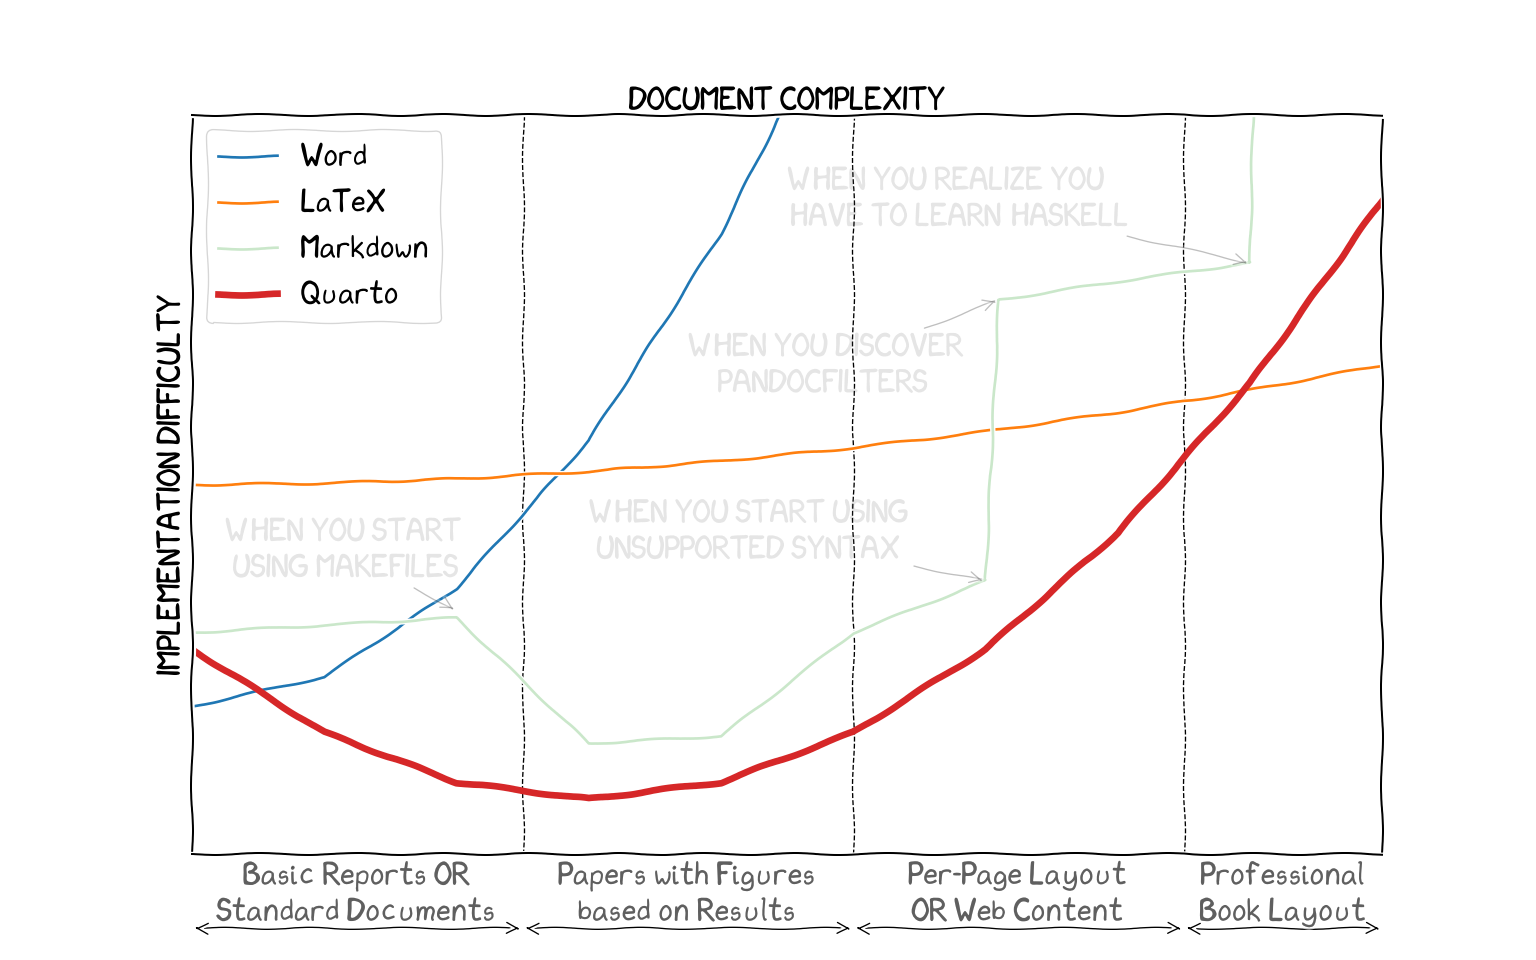
\includegraphics{images/learningcurve.png}
\caption{Comparing Word, \(\LaTeX\) and
Markdown}\label{fig:learningcurve}
}
\end{figure}

If you have gotten this far in the post, congratulations! This was a lot
to take in, and I hope I shed some light on the potential for Markdown
as an academic and technical writing tool. Let me know if you have any
questions in the comments below.

\hypertarget{refs}{}
\begin{cslreferences}
\leavevmode\hypertarget{ref-stallman_emacs_nodate}{}%
{[}1{]} R. Stallman, ``Emacs as word processor.'' Accessed: Jan. 07,
2016. {[}Online{]}. Available:
\url{http://lists.gnu.org/archive/html/emacs-devel/2013-11/msg00515.html}.

\leavevmode\hypertarget{ref-beaumont_bypass_2015}{}%
{[}2{]} K. Beaumont, ``Bypass almost every Corporate security control
with a point'n'click GUI.'' Dec. 2015, Accessed: Jan. 07, 2016.
{[}Online{]}. Available:
\url{https://medium.com/@networksecurity/oleoutlook-bypass-almost-every-corporate-security-control-with-a-point-n-click-gui-37f4cbc107d0}.

\leavevmode\hypertarget{ref-steingold_proprietary_nodate}{}%
{[}3{]} S. Steingold, ``Proprietary Binary Data Formats: Just Say No!''
Accessed: Jan. 07, 2016. {[}Online{]}. Available:
\url{http://www.podval.org/~sds/data.html}.

\leavevmode\hypertarget{ref-cottrell_word_nodate}{}%
{[}4{]} A. Cottrell, ``Word Processors: Stupid and Inefficient.''
Accessed: Jan. 07, 2016. {[}Online{]}. Available:
\url{http://ricardo.ecn.wfu.edu/~cottrell/wp.html}.

\leavevmode\hypertarget{ref-noauthor_stackoverflow_nodate}{}%
{[}5{]} ``StackOverflow Quote.'' Accessed: Jan. 08, 2016. {[}Online{]}.
Available: \url{http://tex.stackexchange.com/a/95078}.

\leavevmode\hypertarget{ref-noauthor_wikibooks_nodate}{}%
{[}6{]} ``Wikibooks LaTeX Tables.'' Accessed: Jan. 07, 2016.
{[}Online{]}. Available:
\url{https://en.wikibooks.org/wiki/LaTeX/Tables}.

\leavevmode\hypertarget{ref-noauthor_github_nodate}{}%
{[}7{]} ``Github repository to Pandoc.'' Accessed: Jan. 06, 2016.
{[}Online{]}. Available: \url{https://github.com/jgm/pandoc/releases}.

\leavevmode\hypertarget{ref-krishnamurthy_github_nodate}{}%
{[}8{]} D. Krishnamurthy, ``Github repository for jupyter notebook
pandocfilter.'' Accessed: Jan. 08, 2016. {[}Online{]}. Available:
\url{https://github.com/kdheepak/pandoc-ipynb}.

\leavevmode\hypertarget{ref-krishnamurthy_using_nodate}{}%
{[}9{]} D. Krishnamurthy, ``Using conda to manage packages.'' Accessed:
Jan. 06, 2016. {[}Online{]}. Available:
\url{http://kdheepak.com/blog/using-conda-to-manage-packages.html}.

\leavevmode\hypertarget{ref-healy_plain_nodate}{}%
{[}10{]} K. Healy, ``Plain Text, Papers, Pandoc.'' {[}Online{]}.
Available:
\url{http://kieranhealy.org/blog/archives/2014/01/23/plain-text/}.

\leavevmode\hypertarget{ref-noauthor_writing_nodate}{}%
{[}11{]} ``Writing academic papers in Markdown using Pandoc.'' Accessed:
Jan. 09, 2016. {[}Online{]}. Available:
\url{http://blog.cigrainger.com/2014/07/pandoc-markdown.html}.

\leavevmode\hypertarget{ref-noauthor_writing_nodate-1}{}%
{[}12{]} ``Writing academic papers in plain text with Markdown and
Jupyter notebook.'' Accessed: Jan. 09, 2016. {[}Online{]}. Available:
\url{http://sylvaindeville.net/2015/07/17/writing-academic-papers-in-plain-text-with-markdown-and-jupyter-notebook/}.

\leavevmode\hypertarget{ref-noauthor_academic_nodate}{}%
{[}13{]} ``Academic Markdown and Citations.'' Accessed: Jan. 09, 2016.
{[}Online{]}. Available:
\url{http://www.chriskrycho.com/2015/academic-markdown-and-citations.html}.

\leavevmode\hypertarget{ref-krishnamurthy_github_nodate-1}{}%
{[}14{]} D. Krishnamurthy, ``Github repository to Pandoc Paper
Template.'' Accessed: Jan. 06, 2016. {[}Online{]}. Available:
\url{https://github.com/kdheepak/pandoc-paper}.

\leavevmode\hypertarget{ref-citation_example}{}%
{[}15{]} J. Doe, ``Example Citation.''.

\leavevmode\hypertarget{ref-noauthor_pandoc_nodate}{}%
{[}16{]} ``Pandoc cross references Github issue tracker.'' {[}Online{]}.
Available: \url{https://github.com/jgm/pandoc/issues/813}.

\leavevmode\hypertarget{ref-noauthor_googlegroups_nodate}{}%
{[}17{]} ``GoogleGroups.'' Accessed: Jan. 08, 2016. {[}Online{]}.
Available:
\url{https://groups.google.com/d/msg/pandoc-discuss/_KyoGN1Zf5g/rzq367675ecJ}.

\leavevmode\hypertarget{ref-duck_github_nodate}{}%
{[}18{]} T. Duck, ``Github repositories of Tom Duck.'' Accessed: Jan.
09, 2016. {[}Online{]}. Available: \url{https://github.com/tomduck}.

\leavevmode\hypertarget{ref-noauthor_pandoc_nodate-1}{}%
{[}19{]} ``Pandoc README.'' Accessed: Jan. 08, 2016. {[}Online{]}.
Available: \url{http://pandoc.org/README.html}.
\end{cslreferences}




\end{document}
